%% LyX 2.1.0 created this file.  For more info, see http://www.lyx.org/.
%% Do not edit unless you really know what you are doing.
\documentclass[english,nojss]{jss}\usepackage[]{graphicx}\usepackage[]{color}
%% maxwidth is the original width if it is less than linewidth
%% otherwise use linewidth (to make sure the graphics do not exceed the margin)
\makeatletter
\def\maxwidth{ %
  \ifdim\Gin@nat@width>\linewidth
    \linewidth
  \else
    \Gin@nat@width
  \fi
}
\makeatother

\definecolor{fgcolor}{rgb}{0.345, 0.345, 0.345}
\newcommand{\hlnum}[1]{\textcolor[rgb]{0.686,0.059,0.569}{#1}}%
\newcommand{\hlstr}[1]{\textcolor[rgb]{0.192,0.494,0.8}{#1}}%
\newcommand{\hlcom}[1]{\textcolor[rgb]{0.678,0.584,0.686}{\textit{#1}}}%
\newcommand{\hlopt}[1]{\textcolor[rgb]{0,0,0}{#1}}%
\newcommand{\hlstd}[1]{\textcolor[rgb]{0.345,0.345,0.345}{#1}}%
\newcommand{\hlkwa}[1]{\textcolor[rgb]{0.161,0.373,0.58}{\textbf{#1}}}%
\newcommand{\hlkwb}[1]{\textcolor[rgb]{0.69,0.353,0.396}{#1}}%
\newcommand{\hlkwc}[1]{\textcolor[rgb]{0.333,0.667,0.333}{#1}}%
\newcommand{\hlkwd}[1]{\textcolor[rgb]{0.737,0.353,0.396}{\textbf{#1}}}%

\usepackage{framed}
\makeatletter
\newenvironment{kframe}{%
 \def\at@end@of@kframe{}%
 \ifinner\ifhmode%
  \def\at@end@of@kframe{\end{minipage}}%
  \begin{minipage}{\columnwidth}%
 \fi\fi%
 \def\FrameCommand##1{\hskip\@totalleftmargin \hskip-\fboxsep
 \colorbox{shadecolor}{##1}\hskip-\fboxsep
     % There is no \\@totalrightmargin, so:
     \hskip-\linewidth \hskip-\@totalleftmargin \hskip\columnwidth}%
 \MakeFramed {\advance\hsize-\width
   \@totalleftmargin\z@ \linewidth\hsize
   \@setminipage}}%
 {\par\unskip\endMakeFramed%
 \at@end@of@kframe}
\makeatother

\definecolor{shadecolor}{rgb}{.97, .97, .97}
\definecolor{messagecolor}{rgb}{0, 0, 0}
\definecolor{warningcolor}{rgb}{1, 0, 1}
\definecolor{errorcolor}{rgb}{1, 0, 0}
\newenvironment{knitrout}{}{} % an empty environment to be redefined in TeX

\usepackage{alltt}
\usepackage[T1]{fontenc}
\usepackage[latin9]{inputenc}
\usepackage{amssymb}
\usepackage[authoryear]{natbib}

\makeatletter
%%%%%%%%%%%%%%%%%%%%%%%%%%%%%% Textclass specific LaTeX commands.
 %\usepackage{Sweave}

%%%%%%%%%%%%%%%%%%%%%%%%%%%%%% User specified LaTeX commands.

\usepackage{amsmath}
\usepackage{nameref}

%the following commands are used only for articles and codesnippets

\author{Matthieu Stigler\\Affiliation IHEID}
\title{\pkg{RDDtools}: an overview }

% the same as above, without any formatting
\Plainauthor{Matthieu Stigler}
\Plaintitle{\pkg{RDDtools}: a toolbox to practice } 
%if necessary, provide a short title
\Shorttitle{\pkg{RDDtools}: a toolbox to practice }

\Abstract{\pkg{RDDtools} is a R package for sharp regression discontinuity design (RDD). It offers various estimators, tests and graphical procedures following the guidelines of  \citet{ImbensLemieux2008} and \citet{LeeLemieux2010}. This note illustrate how to use the package, using the well-known dataset of \citet{Lee2008}.


NOTE THAT this is a preliminary note, on a preliminary package still under  development. Changes of the function names, arguments and output are to be expected, as well as possible mistakes and inconsistencies. Please report any mistakes or suggestion to \email{Matthieu.Stigler@iheid.ch}}
%at least one keyword is needed
\Keywords{Regression discontinuity design, non-parametric analysis, \pkg{RDDtools}, \proglang{R}}
%the same as above, without any formatting
\Plainkeywords{Regression discontinuity design, non-parametric analysis,RDDtools, R} 

%the following commands are used only for book or software reviews

%\Reviewer{Some Author\\University of Somewhere}
%\Plainreviewer{Some Author}

%the following commands are used only for book reviews
%\Booktitle{LyX and \proglang{R}: Secrets of the LyX Master}
%\Bookauthor{Book Author}
%\Pubyear{2008}
%\ISBN{0-12345-678-9}
%\Pages{500}

%the following command is used only for software reviews
%\Softwaretitle{\proglang{gretl 1.7.4}}

%the following commands are used only for book or software reviews
%\Publisher{LyX Publishing Inc.}
%\Pubaddress{LyX City}
%\Price{USD 59.95 (P), USD 99.95 (H)}
%\URL{http://www.lyx.org/}

%without any formatting
%\Plaintitle{LyX and R: Secrets of the LyX Master}
%\Shorttitle{LyX and R}

%the following commands are used for articles, codesnippets, book reviews and software reviews

%publication information
%do not use these commands before the article has been accepted
%\Volume{00}
%\Issue{0}
%\Month{Month}
%\Year{2000}
%\Submitdate{2000-00-00}
%\Acceptdate{2000-00-00}

%The address of at least one author should be given in the following format
\Address{
  Matthieu Stigler\\
  Centre for Finance and development\\
  IHEID\\
  Geneva\\
  E-mail: \email{Matthieu.Stigler@iheid.ch}
}
%you can add a telephone and fax number before the e-mail in the format
%Telephone: +12/3/4567-89
%Fax: +12/3/4567-89

%if you use Sweave,  include the following line (with % symbols):
%% need no \usepackage{Sweave.sty}

%% Arg min operator:
\DeclareMathOperator*{\argmi}{arg\,min}
\newcommand{\argmin}[1]{\underset{#1}{\argmi}}

\DeclareMathOperator*{\Ker}{\mathcal{K}}

\makeatother

\usepackage{babel}
\IfFileExists{upquote.sty}{\usepackage{upquote}}{}
\begin{document}
\tableofcontents{}


\section{Introduction}

\addcontentsline{toc}{section}{Introduction}


\subsection{Introduction to RDD}




\subsection{Introduction to RDDtools}

The R package \pkg{RDDtools} aims at offering a complete a toolbox
for regression discontinuity design, following the step-by-step recommendations
of \citet{ImbensLemieux2008} and \citet{LeeLemieux2010}. Summarising
the approaches advocated in the two papers, a RDD analysis comprises
of following steps:
\begin{enumerate}
\item Graphical representation of the data
\item Estimation 
\item Validity tests
\end{enumerate}
We add to this list a step that is too often forgotten, yet can be
very burdensome: data preparation. Hence, this list is extended with
the fundamental step 0, which involves preparing the data in the right
way. 

\pkg{RDDtools} offers an object-oriented way to analysis, building
on the R mechanism of S3 methods and classes. Concretely, this implies
that the user has to specify the input data only once, and that most
of the functions can be called directly on the new object of class
\code{RDDdata}.


\section{Step 0: data input}

\addcontentsline{toc}{section}{Step 0: data input}

As first step of the analysis, the user has to specify the input data
into the \code{RDDdata} function, which takes following arguments:
\begin{description}
\item [{y}] The outcome variable
\item [{x}] The forcing variable 
\item [{cutpoint}] The cutpoint/threshold (note only one cutpoint can be
given)
\item [{covar}] Eventual covariates
\end{description}
The RDDdata function returns an object of class \code{RDDdata}, as
well as of the usual \proglang{R} class \code{data.frame}. 

To illustrate this, we show how to use this with the benchmark dataset
of \citet{Lee2008}, adding randomly generated covariates for the
sake of illustration. The dataset is shipped with the package, and
is available under the name \emph{Lee2008. }Using the R \code{head}
function, we look at the first rows of the dataset:

\begin{knitrout}
\definecolor{shadecolor}{rgb}{0.969, 0.969, 0.969}\color{fgcolor}\begin{kframe}
\begin{alltt}
\hlkwd{library}\hlstd{(RDDtools)}
\hlkwd{data}\hlstd{(Lee2008)}
\hlkwd{head}\hlstd{(Lee2008)}
\end{alltt}
\begin{verbatim}
##         x      y
## 1  0.1049 0.5810
## 2  0.1393 0.4611
## 3 -0.0736 0.5434
## 4  0.0868 0.5846
## 5  0.3994 0.5803
## 6  0.1681 0.6244
\end{verbatim}
\end{kframe}
\end{knitrout}


The data is already clean, so the only step required is to fit it
into the RDDdata function, adding however the information on the cutpoint.
For illustration purpose, we add also some random covariates as a
matrix Z:

\begin{knitrout}
\definecolor{shadecolor}{rgb}{0.969, 0.969, 0.969}\color{fgcolor}\begin{kframe}
\begin{alltt}
\hlstd{n_Lee} \hlkwb{<-} \hlkwd{nrow}\hlstd{(Lee2008)}
\hlstd{Z} \hlkwb{<-} \hlkwd{data.frame}\hlstd{(}\hlkwc{z1} \hlstd{=} \hlkwd{rnorm}\hlstd{(n_Lee),} \hlkwc{z2} \hlstd{=} \hlkwd{rnorm}\hlstd{(n_Lee,} \hlkwc{mean} \hlstd{=} \hlnum{20}\hlstd{,} \hlkwc{sd} \hlstd{=} \hlnum{2}\hlstd{),} \hlkwc{z3} \hlstd{=} \hlkwd{sample}\hlstd{(letters[}\hlnum{1}\hlopt{:}\hlnum{3}\hlstd{],}
    \hlkwc{size} \hlstd{= n_Lee,} \hlkwc{replace} \hlstd{=} \hlnum{TRUE}\hlstd{))}
\hlstd{Lee2008_rdd} \hlkwb{<-} \hlkwd{RDDdata}\hlstd{(}\hlkwc{y} \hlstd{= Lee2008}\hlopt{$}\hlstd{y,} \hlkwc{x} \hlstd{= Lee2008}\hlopt{$}\hlstd{x,} \hlkwc{covar} \hlstd{= Z,} \hlkwc{cutpoint} \hlstd{=} \hlnum{0}\hlstd{)}
\end{alltt}
\end{kframe}
\end{knitrout}


We now have an object \code{Lee2008_rdd} of class \code{RDDdata}
(and \code{data.frame}). It has a specific \code{summary} method,
which gives a few summary informations about the dataset:

\begin{knitrout}
\definecolor{shadecolor}{rgb}{0.969, 0.969, 0.969}\color{fgcolor}\begin{kframe}
\begin{alltt}
\hlkwd{summary}\hlstd{(Lee2008_rdd)}
\end{alltt}
\begin{verbatim}
## ### RDDdata object ###
## 
## Cutpoint: 0 
## Sample size: 
## 	-Full : 6558 
## 	-Left : 2740 
## 	-Right: 3818
## Covariates: yes
\end{verbatim}
\end{kframe}
\end{knitrout}


Another function for \code{RDDdata} objects is the \code{plot()}
function, discussed in the next section. 


\section{Step 1: Graphical representation}

\addcontentsline{toc}{section}{Step 1: Graphical representation}

Once the dataset has been formatted with the RDDdata function, it
can be used directly for simple illustration. Indeed, as recommended
by \citet{LeeLemieux2010}, it is always good to show the raw data
first, if ones wishes to convince that there is a discontinuity. This
is simply done using the standard R plot() function, which has been
customised for RDDdata objects. The function shows a scatter plot
of the outcome variable against the forcing variable. Following \citet{LeeLemieux2010},
not all single datapoints are shown: instead, a ``binned'' scatterplot
is shown, using non-overlapping averages:

\begin{knitrout}
\definecolor{shadecolor}{rgb}{0.969, 0.969, 0.969}\color{fgcolor}\begin{kframe}
\begin{alltt}
\hlkwd{plot}\hlstd{(Lee2008_rdd)}
\end{alltt}
\end{kframe}
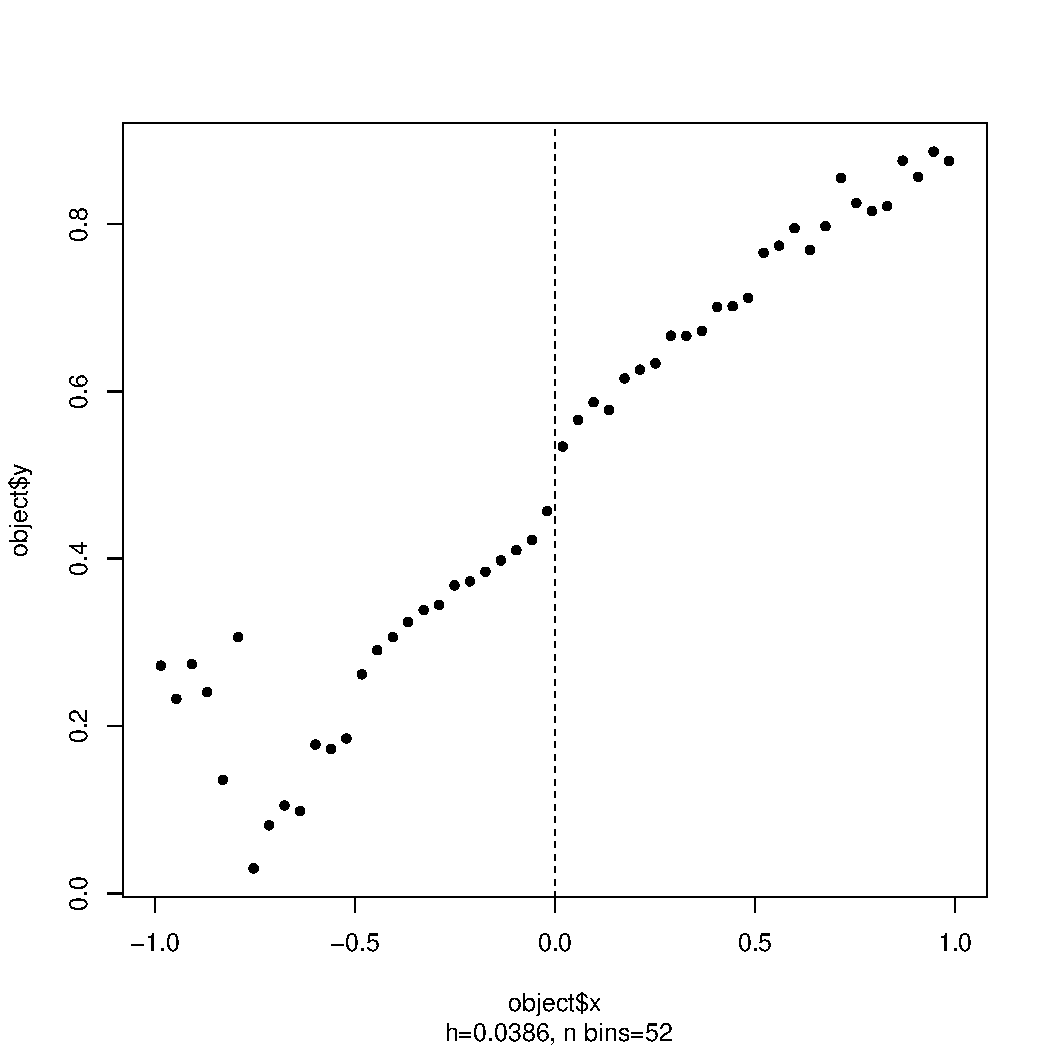
\includegraphics[width=\maxwidth]{figure/unnamed-chunk-4} 

\end{knitrout}


The bandwidth for the bins (also called binwidth) can be set by the
user with the \code{h} argument. If this it is not provided by the
user, the function uses by default the global bandwidth of \citet{RuppertSheatherEtAl1995},
implemented in the \code{RDDbw_RSW()} function. 

Another argument that might be useful for the user is the option \code{nplot},
which allows to plot multiple plots with different bandwidths:

\begin{knitrout}
\definecolor{shadecolor}{rgb}{0.969, 0.969, 0.969}\color{fgcolor}\begin{kframe}
\begin{alltt}
\hlkwd{plot}\hlstd{(Lee2008_rdd,} \hlkwc{nplot} \hlstd{=} \hlnum{3}\hlstd{,} \hlkwc{h} \hlstd{=} \hlkwd{c}\hlstd{(}\hlnum{0.02}\hlstd{,} \hlnum{0.03}\hlstd{,} \hlnum{0.04}\hlstd{))}
\end{alltt}
\end{kframe}
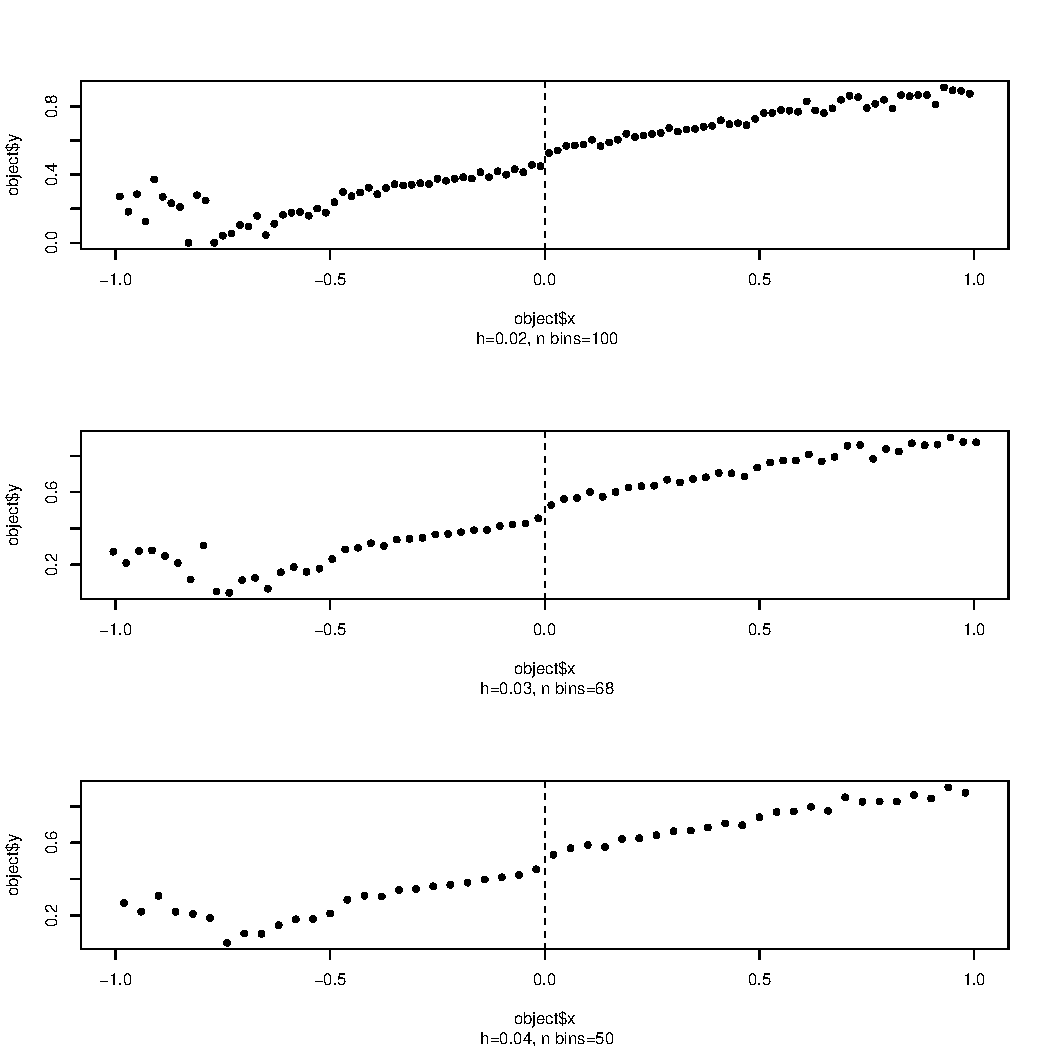
\includegraphics[width=\maxwidth]{figure/unnamed-chunk-5} 

\end{knitrout}


Note however that experience shows that showing multiple plots have
the effect to shrink considerably the y axis, reducing the visual
impression of discontinuity. 


\section{Step 2: Estimation}

\addcontentsline{toc}{section}{Step 2: Estimation}

RDDtools offers currently two estimators:
\begin{itemize}
\item the simple parametric estimator: function \code{RDDreg_lm()}. 
\item the non-parametric local-linear estimator: function \code{RDDreg_np()}. 
\end{itemize}
These two functions share some common arguments, which are:
\begin{description}
\item [{RDDobject:}] the input data as obtained with the \code{RDDdata()}
function
\item [{bw:}] the bandwidth. 
\item [{covariates:}] this will allow to add covariates in the analysis.
Note that it is presently NOT used. 
\end{description}
The bandwidth argument has a different behaviour in the parametric
and non-parametric way: while the parametric estimation can be done
without bandwidth, the non-parametric estimator is by definition based
on a bandwidth. This means that the default behaviours are different:
if no bandwidth is given for the parametric model, the model will
be simply estimated withut bandwidth, that is covering the full sample
on both sides of the cutpoint. On the other side, if no bandwidth
is provided in the non-parametric case, a bandwidth will still be
computed automatically using the method advocated by \citet{ImbensKalyanaraman2012}. 


\subsection{Parametric}

The parametric estimator simply estimates a function over the whole
sample (hence called \emph{pooled regression} by \citealp{LeeLemieux2010}):

\begin{equation}
Y=\alpha+\tau D+\beta(X-c)+\epsilon\label{eq:ParamStandard}
\end{equation}


where D is a dummy variable, indicating whether the observations are
above (or equal to) the cutoff point, i.e. $D=I(X\geq c)$. The parameter
of interest is $\tau$, which represents the difference in intercepts
$\alpha_{r}-\alpha_{l}$, i.e. the discontinuity. Note that equation
\ref{eq:ParamStandard} imposes the slope to be equal on both sides
of the cutoff point. While such restriction should hold locally around
the threshold (due to the assumption of random assignment around the
cutoff point), the parametric regression is done by default using
the whole sample, so the restriction is unlikely to hold. In this
case, one should rather estimate:

\begin{equation}
Y=\alpha+\tau D+\beta_{1}(X-c)+\beta_{2}D(X-c)+\epsilon\label{eq:Param2slopes}
\end{equation}


so that $\beta_{1}=\beta_{l}$, and $\beta_{2}=\beta_{r}-\beta_{l}$. 

The two estimators are available with the \code{RDDreg_lm()} function,
the choice between the specifications being made through the \code{slope=c("separate", "same")}
argument:
\begin{description}
\item [{separate:}] the default, estimates different slopes, i.e. equation~\ref{eq:Param2slopes}.
\item [{same:}] Estimates a common slope, i.e. equation~\ref{eq:ParamStandard}.
\end{description}
Note that the order of X has been set as 1 in both cases. If the function
shows moderate non-linearity, this can be potentially captured by
adding further power of X, leading to (for the separate slope equation:)

\begin{equation}
Y=\alpha+\tau D+\beta_{1}^{1}(X-c)+\beta_{2}^{1}D(X-c)+\ldots+\beta_{1}^{p}(X-c)^{p}+\beta_{2}^{p}D(X-c)^{p}+\epsilon\label{eq:ParamSlopesPowers}
\end{equation}


The order of the polynomial can be adjusted with the \code{order}
argument. 

Finally, the estimator can be restricted to a (symmetric) window around
the cutoff point, as is done usually in practice. This is done using
the \code{bw} option. 

In summary, the function \code{RDDreg_lm()} has three main options: 
\begin{description}
\item [{slope:}] Whether to use different slopes on each side of the cutoff
(default) or not.
\item [{order:}] Order of the polynomial in X. Default to 1.
\item [{bw:}] Eventual window to estimate the data. Default to full data. 
\end{description}
We show now the different applications, still using the Lee dataset:

\begin{knitrout}
\definecolor{shadecolor}{rgb}{0.969, 0.969, 0.969}\color{fgcolor}\begin{kframe}
\begin{alltt}
\hlstd{reg_linear_1} \hlkwb{<-} \hlkwd{RDDreg_lm}\hlstd{(Lee2008_rdd)}
\end{alltt}
\end{kframe}
\end{knitrout}


We now estimate different versions, first restricting the slope to
be the same, then changing the order, and finally using a smaller
window:

\begin{knitrout}
\definecolor{shadecolor}{rgb}{0.969, 0.969, 0.969}\color{fgcolor}\begin{kframe}
\begin{alltt}
\hlstd{reg_linear_2} \hlkwb{<-} \hlkwd{RDDreg_lm}\hlstd{(Lee2008_rdd,} \hlkwc{slope} \hlstd{=} \hlstr{"same"}\hlstd{)}
\hlstd{reg_linear_3} \hlkwb{<-} \hlkwd{RDDreg_lm}\hlstd{(Lee2008_rdd,} \hlkwc{order} \hlstd{=} \hlnum{3}\hlstd{)}
\hlstd{reg_linear_4} \hlkwb{<-} \hlkwd{RDDreg_lm}\hlstd{(Lee2008_rdd,} \hlkwc{bw} \hlstd{=} \hlnum{0.4}\hlstd{)}
\end{alltt}
\end{kframe}
\end{knitrout}


Model's output is shown with the \code{print()} and \code{summary()}
function: while the \code{print()} function just shows few informations
and the LATE estimate, the \code{summary()} function shows the full
output of the underlying regression model:

\begin{knitrout}
\definecolor{shadecolor}{rgb}{0.969, 0.969, 0.969}\color{fgcolor}\begin{kframe}
\begin{alltt}
\hlstd{reg_linear_1}
\end{alltt}
\begin{verbatim}
## ### RDD regression: parametric ###
## 	Polynomial order:  1 
## 	Slopes:  separate 
## 	Number of obs: 6558 (left: 2740, right: 3818)
## 
## 	Coefficient:
##   Estimate Std. Error t value Pr(>|t|)    
## D  0.11823    0.00568    20.8   <2e-16 ***
## ---
## Signif. codes:  0 '***' 0.001 '**' 0.01 '*' 0.05 '.' 0.1 ' ' 1
\end{verbatim}
\begin{alltt}
\hlkwd{summary}\hlstd{(reg_linear_1)}
\end{alltt}
\begin{verbatim}
## 
## Call:
## lm(formula = y ~ ., data = dat_step1, weights = weights)
## 
## Residuals:
##     Min      1Q  Median      3Q     Max 
## -0.8941 -0.0619  0.0023  0.0713  0.8640 
## 
## Coefficients:
##             Estimate Std. Error t value Pr(>|t|)    
## (Intercept)  0.43295    0.00428  101.25  < 2e-16 ***
## D            0.11823    0.00568   20.82  < 2e-16 ***
## x            0.29691    0.01155   25.71  < 2e-16 ***
## x_right      0.04598    0.01350    3.41  0.00066 ***
## ---
## Signif. codes:  0 '***' 0.001 '**' 0.01 '*' 0.05 '.' 0.1 ' ' 1
## 
## Residual standard error: 0.138 on 6554 degrees of freedom
## Multiple R-squared:  0.671,	Adjusted R-squared:  0.671 
## F-statistic: 4.45e+03 on 3 and 6554 DF,  p-value: <2e-16
\end{verbatim}
\begin{alltt}
\hlstd{reg_linear_2}
\end{alltt}
\begin{verbatim}
## ### RDD regression: parametric ###
## 	Polynomial order:  1 
## 	Slopes:  same 
## 	Number of obs: 6558 (left: 2740, right: 3818)
## 
## 	Coefficient:
##   Estimate Std. Error t value Pr(>|t|)    
## D  0.11373    0.00553    20.6   <2e-16 ***
## ---
## Signif. codes:  0 '***' 0.001 '**' 0.01 '*' 0.05 '.' 0.1 ' ' 1
\end{verbatim}
\begin{alltt}
\hlstd{reg_linear_3}
\end{alltt}
\begin{verbatim}
## ### RDD regression: parametric ###
## 	Polynomial order:  3 
## 	Slopes:  separate 
## 	Number of obs: 6558 (left: 2740, right: 3818)
## 
## 	Coefficient:
##   Estimate Std. Error t value Pr(>|t|)    
## D   0.1115     0.0107    10.5   <2e-16 ***
## ---
## Signif. codes:  0 '***' 0.001 '**' 0.01 '*' 0.05 '.' 0.1 ' ' 1
\end{verbatim}
\begin{alltt}
\hlstd{reg_linear_4}
\end{alltt}
\begin{verbatim}
## ### RDD regression: parametric ###
## 	Polynomial order:  1 
## 	Slopes:  separate 
## 	Bandwidth:  0.4 
## 	Number of obs: 4169 (left: 2043, right: 2126)
## 
## 	Coefficient:
##   Estimate Std. Error t value Pr(>|t|)    
## D  0.08863    0.00727    12.2   <2e-16 ***
## ---
## Signif. codes:  0 '***' 0.001 '**' 0.01 '*' 0.05 '.' 0.1 ' ' 1
\end{verbatim}
\end{kframe}
\end{knitrout}


Finally, a \code{plot()} function adds the estimated curve to the
binned plot. Here we show the difference between the model estimated
with polynomial of order 1 and order 3:

\begin{knitrout}
\definecolor{shadecolor}{rgb}{0.969, 0.969, 0.969}\color{fgcolor}\begin{kframe}
\begin{alltt}
\hlkwd{par}\hlstd{(}\hlkwc{mfrow} \hlstd{=} \hlkwd{c}\hlstd{(}\hlnum{2}\hlstd{,} \hlnum{1}\hlstd{))}
\hlkwd{plot}\hlstd{(reg_linear_1)}
\hlkwd{plot}\hlstd{(reg_linear_3)}
\end{alltt}
\end{kframe}
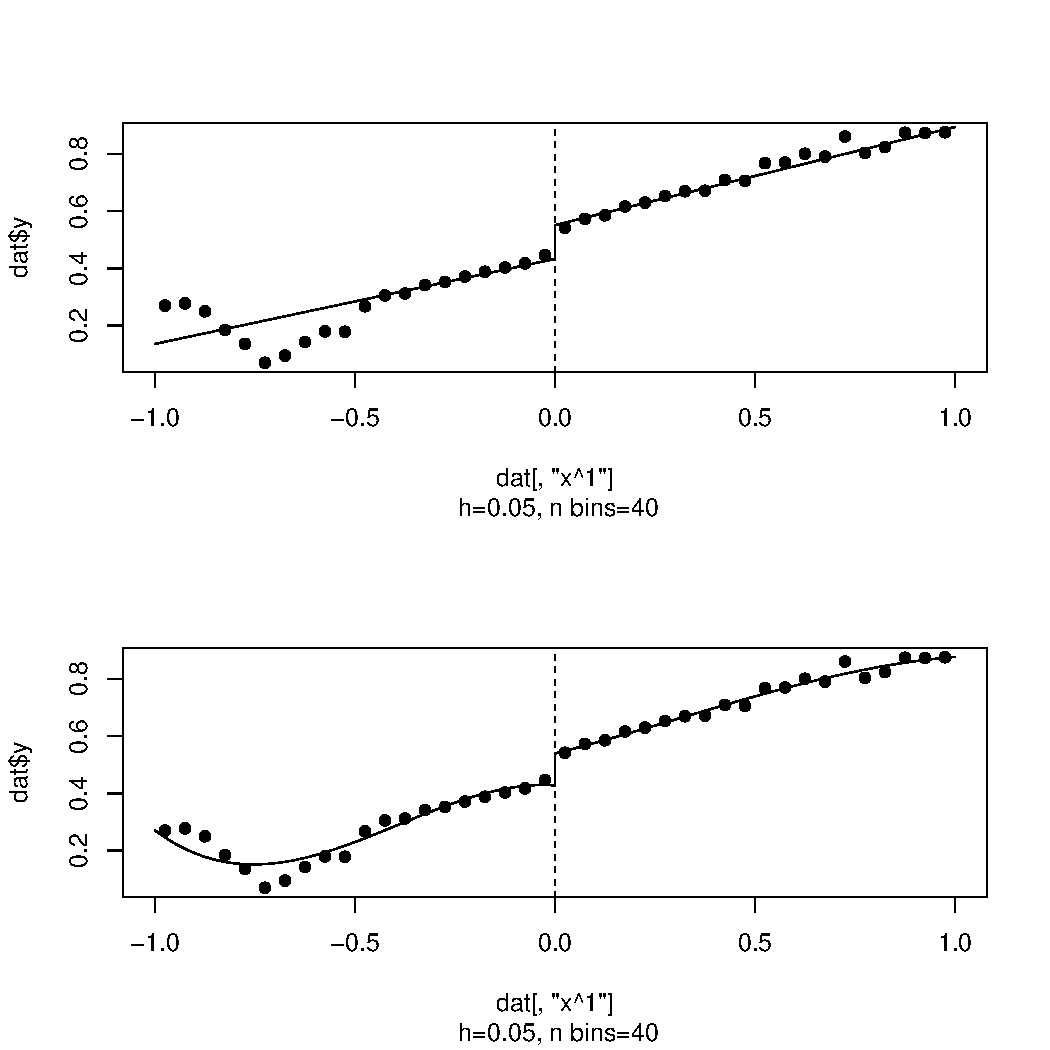
\includegraphics[width=\maxwidth]{figure/unnamed-chunk-9} 
\begin{kframe}\begin{alltt}
\hlkwd{par}\hlstd{(}\hlkwc{mfrow} \hlstd{=} \hlkwd{c}\hlstd{(}\hlnum{1}\hlstd{,} \hlnum{1}\hlstd{))}
\end{alltt}
\end{kframe}
\end{knitrout}



\subsection{Non-parametric}

Although the parametric estimator is often used in practice, another
estimator has important appeal, in this context where one is interested
in estimating a regression just around a cutoff. In this case, non-parametric
estimators such as the local-linear kernel regression of \citet{FanGijbels1992,FanGijbels1996},
which aim at estimating a regression locally at each point, have interesting
features, as advocated by \citet{Porter2003}. A local linear regression
amounts to do a simple weighted linear regression, where the weights
are given by a kernel function. Formally, the local-linear estimator
(LLE) is given by its estimating equation:



\begin{equation}
\hat{\alpha}(c),\hat{\beta}(c),\hat{\tau}(c)=\argmin{\alpha,\beta,\tau}\sum_{i=1}^{n}\left(Y_{i}-\alpha-\tau D-\beta(X_{i}-c)\right)^{2}\mathcal{K}\left(\frac{X_{i}-c}{h}\right)\label{eq:LLEform}
\end{equation}


where $\mathcal{K}(\cdot)$ is a kernel function attributing weights
to each point according to their distance to the point c. Note that
the parameters $\alpha$, $\beta$ and $\tau$ are written as of function
of $c$ to emphasize the fact that these are \emph{local} estimate,
unlike in the parametric rate. The kernel used in RDDtools here is
the triangular kernel (also called \emph{edge} function sometimes):
$K(x)=I(|x|\leq1)(1-|x|)$. This choice, which departs from the the
suggestion of \citet{LeeLemieux2010}, is driven by the fact that
the triangular kernel was shown to be optimal when one estimates a
parameter at a boundary, which is precisely our case here \citep{ChengFanEtAl1997}.
Unlike the package \pkg{rdd}, we do not offer other kernels in \pkg{RDDtools},
since the kernel selected is optimal, and changing the kernel is found
to have little impact compared to changing the bandwidths.

Note that using the LLE estimator reduces to do a weighted OLS (WOLS)
at each point%
\footnote{See \citep[equ. 3.4, page  58]{FanGijbels1996}. %
}, which allows to use the usual regression function \code{lm()} in
R, specifying the weights as given by the kernel. However, although
this is a WOLS, the variance of the LLE is not the same as that of
the WOLS, unless one is ready to assume that the bandwidth used is
the true \emph{bandwidth}%
\footnote{A second option is use a smaller bandwidth, in which case standard
inference can be applied. This has however the drawback of using a
sub-optimal bandwidth, with a slower rate of convergence. %
}. However, most, if not all, papers in the literature do use the standard
WOLS inference, eventually adjusted for heteroskedasticity. This is
also done currently in the RDDtools package, although we intend to
do this following the work of \citet{CalonicoCattaneoEtAl2012}. 

Another question arises is the choice of the bandwidth, which is a
crucial question since this choice has a huge impact on the estimation.
Typically, decreasing the bandwidth will reduce the bias of the estimator,
but increase its variance. One way of choosing the bandwidth is then
to try to minimise the mean-squared error (MSE) of the estimator,
which allows to trade-off bias and variance. This approach is pursued
by \citet{ImbensKalyanaraman2012}, and is available in \pkg{RDDtools}
with the function \code{RDDbw_IK()}. This function takes simply a
RDDdata object as input, and returns the optimal value according to
the MSE criterion. 

As an illustration, we use now the non-parametric estimator for the
Lee dataset, estimating first the bandwidth and then the discontinuity
with \code{RDDreg_np()}:

\begin{knitrout}
\definecolor{shadecolor}{rgb}{0.969, 0.969, 0.969}\color{fgcolor}\begin{kframe}
\begin{alltt}
\hlstd{bw_IK} \hlkwb{<-} \hlkwd{RDDbw_IK}\hlstd{(Lee2008_rdd)}
\hlstd{bw_IK}
\end{alltt}
\begin{verbatim}
##  h_opt 
## 0.2939
\end{verbatim}
\begin{alltt}
\hlstd{reg_nonpara} \hlkwb{<-} \hlkwd{RDDreg_np}\hlstd{(}\hlkwc{RDDobject} \hlstd{= Lee2008_rdd,} \hlkwc{bw} \hlstd{= bw_IK)}
\end{alltt}
\end{kframe}
\end{knitrout}


The output, of class \code{RDDreg_np}, has the usual \code{print()},
\code{summary()} and \code{plot()} functions:

\begin{knitrout}
\definecolor{shadecolor}{rgb}{0.969, 0.969, 0.969}\color{fgcolor}\begin{kframe}
\begin{alltt}
\hlstd{reg_nonpara}
\end{alltt}
\begin{verbatim}
## ### RDD regression: nonparametric local linear###
## 	Bandwidth:  0.2939 
## 	Number of obs: 3200 (left: 1594, right: 1606)
## 
## 	Coefficient:
##   Estimate Std. Error z value Pr(>|z|)    
## D  0.07992    0.00946    8.44   <2e-16 ***
## ---
## Signif. codes:  0 '***' 0.001 '**' 0.01 '*' 0.05 '.' 0.1 ' ' 1
\end{verbatim}
\begin{alltt}
\hlkwd{summary}\hlstd{(reg_nonpara)}
\end{alltt}
\begin{verbatim}
## ### RDD regression: nonparametric local linear###
## 	Bandwidth:  0.2939 
## 	Number of obs: 3200 (left: 1594, right: 1606)
## 
## 	Weighted Residuals:
##     Min      1Q  Median      3Q     Max 
## -0.9775 -0.0672 -0.0050  0.0450  0.9376 
## 
## 	Coefficient:
##   Estimate Std. Error z value Pr(>|z|)    
## D  0.07992    0.00946    8.44   <2e-16 ***
## ---
## Signif. codes:  0 '***' 0.001 '**' 0.01 '*' 0.05 '.' 0.1 ' ' 1
## 
## 	Local R squared: 0.356
\end{verbatim}
\end{kframe}
\end{knitrout}


The \code{plot()} function shows the point estimates%
\footnote{Note that the estimates are obtained with the \code{locpoly()} function
from package \pkg{KernSmooth}. This has however the disadvantage
that it is not the same kernel used as in the previously, since the
locpoly function uses a gaussian kernel, while we use a triangular
one. Since this is only for visual purpose, the difference should
however not be perceptible. Furthermore, using the \code{locpoly()}
function has the advantage that the algorithm is way faster, since
the authors did implement a fast binned implementation, see \citet[section 3.6]{FanGijbels1996}. %
} over a grid defined within the bandwidth range, i.e. the parameter
$\alpha(x)$ from equation~\ref{eq:LLEform} such as $\alpha(x)\quad$$\forall$
$[x-bw;x+bw]$. This should not be confused with the line drawn in
the parametric plots, which show the curve $y=f(x)=\hat{\alpha}+\hat{\beta}(x-c)+\hat{\tau}D$. 

\begin{knitrout}
\definecolor{shadecolor}{rgb}{0.969, 0.969, 0.969}\color{fgcolor}\begin{kframe}
\begin{alltt}
\hlkwd{plot}\hlstd{(reg_nonpara)}
\end{alltt}
\end{kframe}
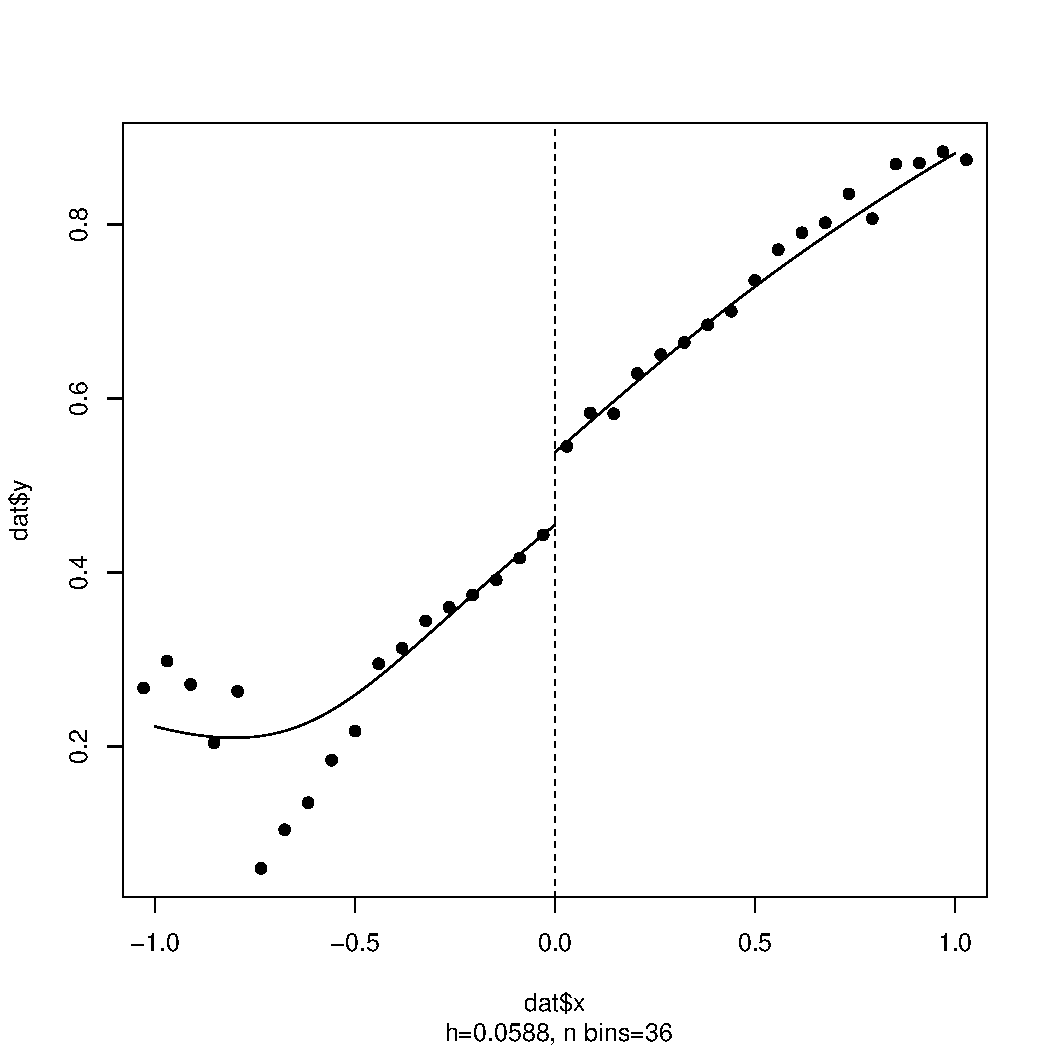
\includegraphics[width=\maxwidth]{figure/unnamed-chunk-12} 

\end{knitrout}



\subsection{Assessing the sensibility of the estimator}

Both the parametric and non-parametric estimators are dependent on
the choice of extra-parameters such as the polynomial order, or the
bandwidth. It is however known that this choice can have a big impact,
especially in the case of the bandwidth choice for the non-parametric
case. A simple way to assess the sensitivity of the results is to
plot the value of the estimate against multiple bandwidths. This is
the purpose of the function \code{plotSensi()}, which work both on
\code{RDDreg_lm()} as well as \code{RDDreg_np()}. In the former
case, the function will assess the sensitivity against the polynomial
order (eventually the bandwidth if it was specified), while in the
latter case against the bandwidth. 

We illustrate this on the previous non-parametric estimator:

\begin{knitrout}
\definecolor{shadecolor}{rgb}{0.969, 0.969, 0.969}\color{fgcolor}\begin{kframe}
\begin{alltt}
\hlkwd{plotSensi}\hlstd{(reg_nonpara,} \hlkwc{device} \hlstd{=} \hlstr{"ggplot"}\hlstd{)}
\end{alltt}
\end{kframe}
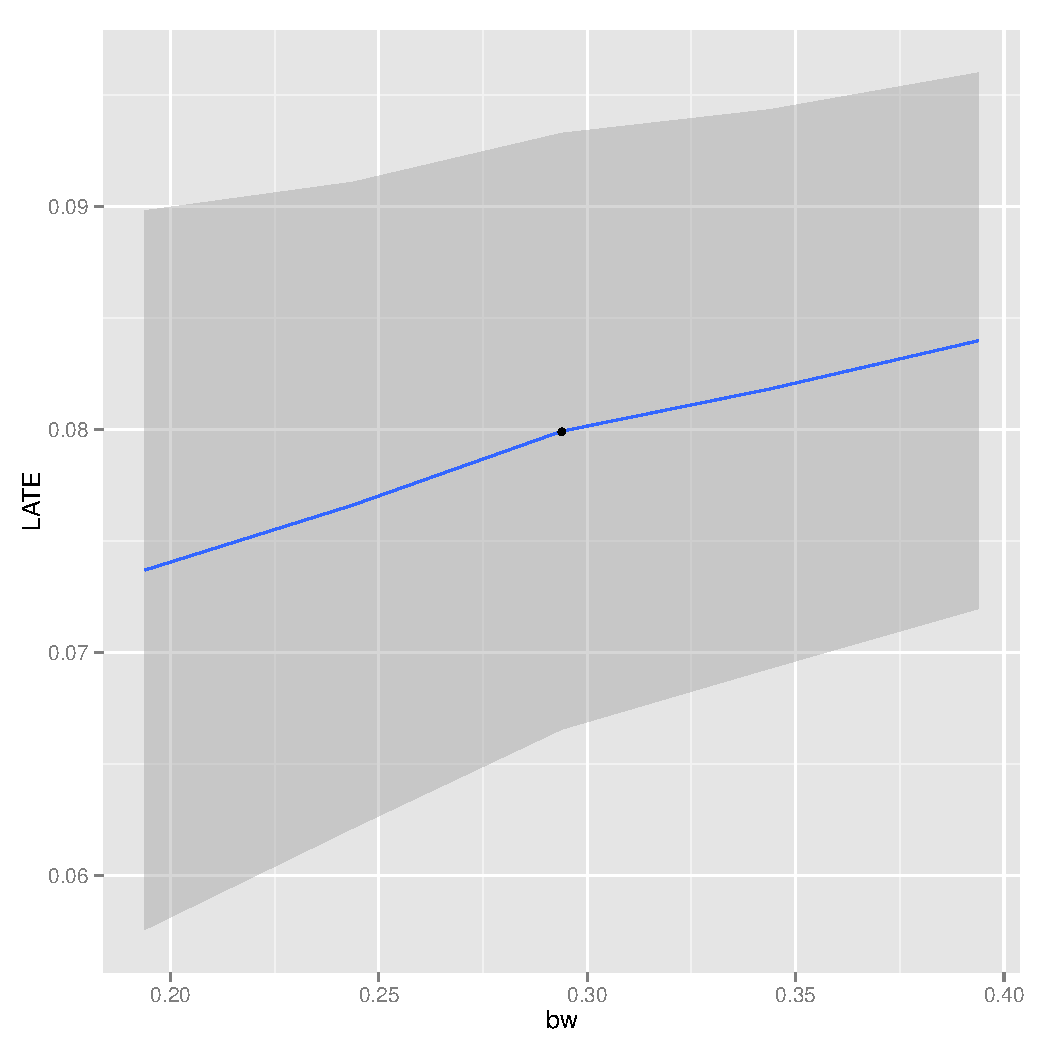
\includegraphics[width=\maxwidth]{figure/unnamed-chunk-13} 

\end{knitrout}


and we illustrate it also on the parametric estimator where a bandwidth
was specified:

\begin{knitrout}
\definecolor{shadecolor}{rgb}{0.969, 0.969, 0.969}\color{fgcolor}\begin{kframe}
\begin{alltt}
\hlkwd{plotSensi}\hlstd{(reg_linear_4,} \hlkwc{device} \hlstd{=} \hlstr{"ggplot"}\hlstd{)}
\end{alltt}
\end{kframe}
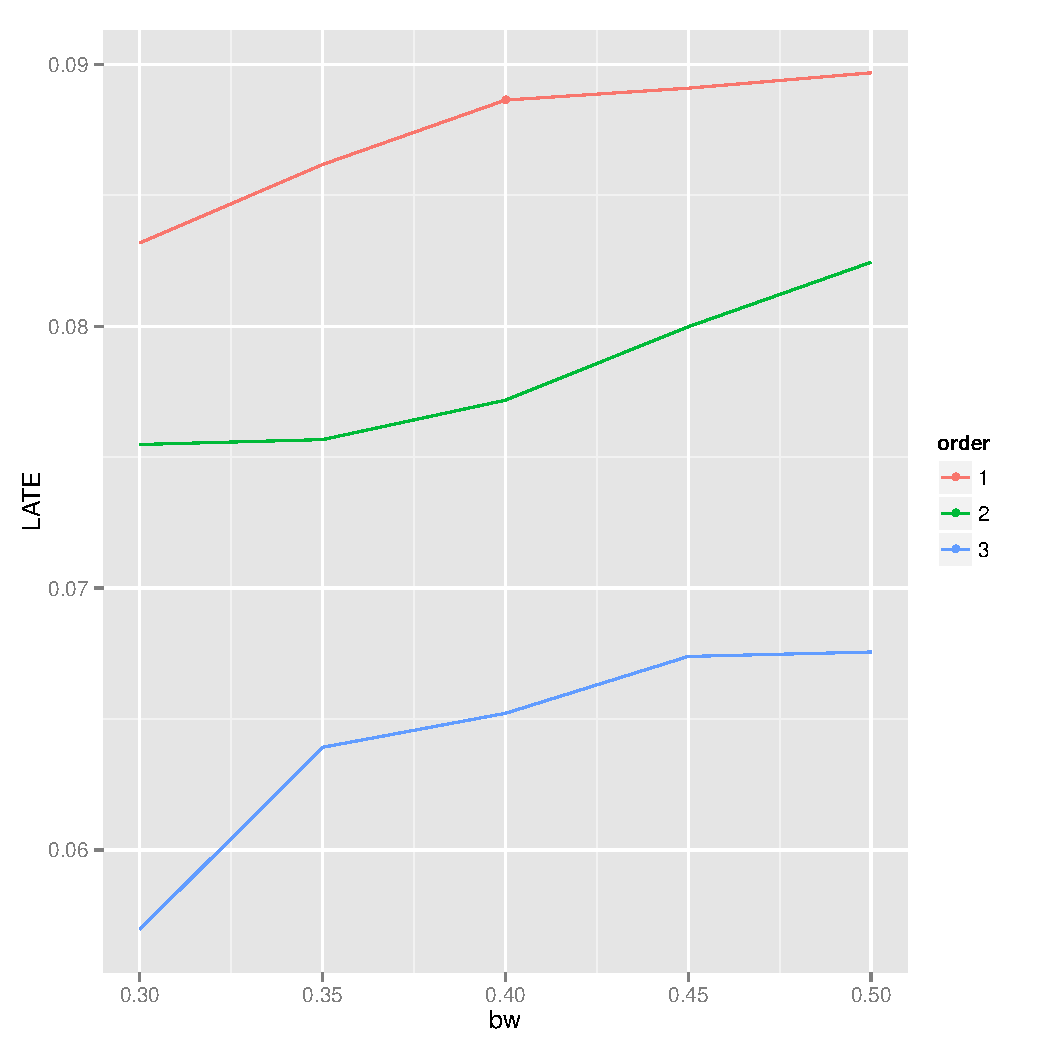
\includegraphics[width=\maxwidth]{figure/unnamed-chunk-14} 

\end{knitrout}



\section{Step 3: Validity tests}

\addcontentsline{toc}{section}{Step 3: Validity tests}

Once the discontinuity estimated and its sensitivity against the bandwidth
choice assessed, the last step in the analysis is to proceed to a
few validity tests. 


\subsection{Placebo tests}

A way to convince its readers that the discontinuity one has found
is a true one is to show that it is not the a spurious result one
could have obtained at a random cutoff. Hence, as advocated by \citet{ImbensLemieux2008},
one can run placebo tests, where one estimates a discontinuity but
at a different point than the true cutoff. This is available through
the \code{plotPlacebo()} function, which works on \code{RDDreg_lm}
or \code{RDDreg_np} objects. An important question is on which point
this should be tested. The fact is that the sample should not contain
the cutoff point (so that the presence of a discontinuity at its point
does not impact the estimates at other points), and be far away from
that cutoff (as well as from the min and max of the whole distribution)
so that it contains a fair amount of points at both sides for estimation.
The default is then to run for points on the left within the first
and last quartiles of the left sample, and the same on the right.

We illustrate this on the non-parametric estimator:

\begin{knitrout}
\definecolor{shadecolor}{rgb}{0.969, 0.969, 0.969}\color{fgcolor}\begin{kframe}
\begin{alltt}
\hlkwd{plotPlacebo}\hlstd{(reg_nonpara,} \hlkwc{device} \hlstd{=} \hlstr{"ggplot"}\hlstd{)}
\end{alltt}
\end{kframe}
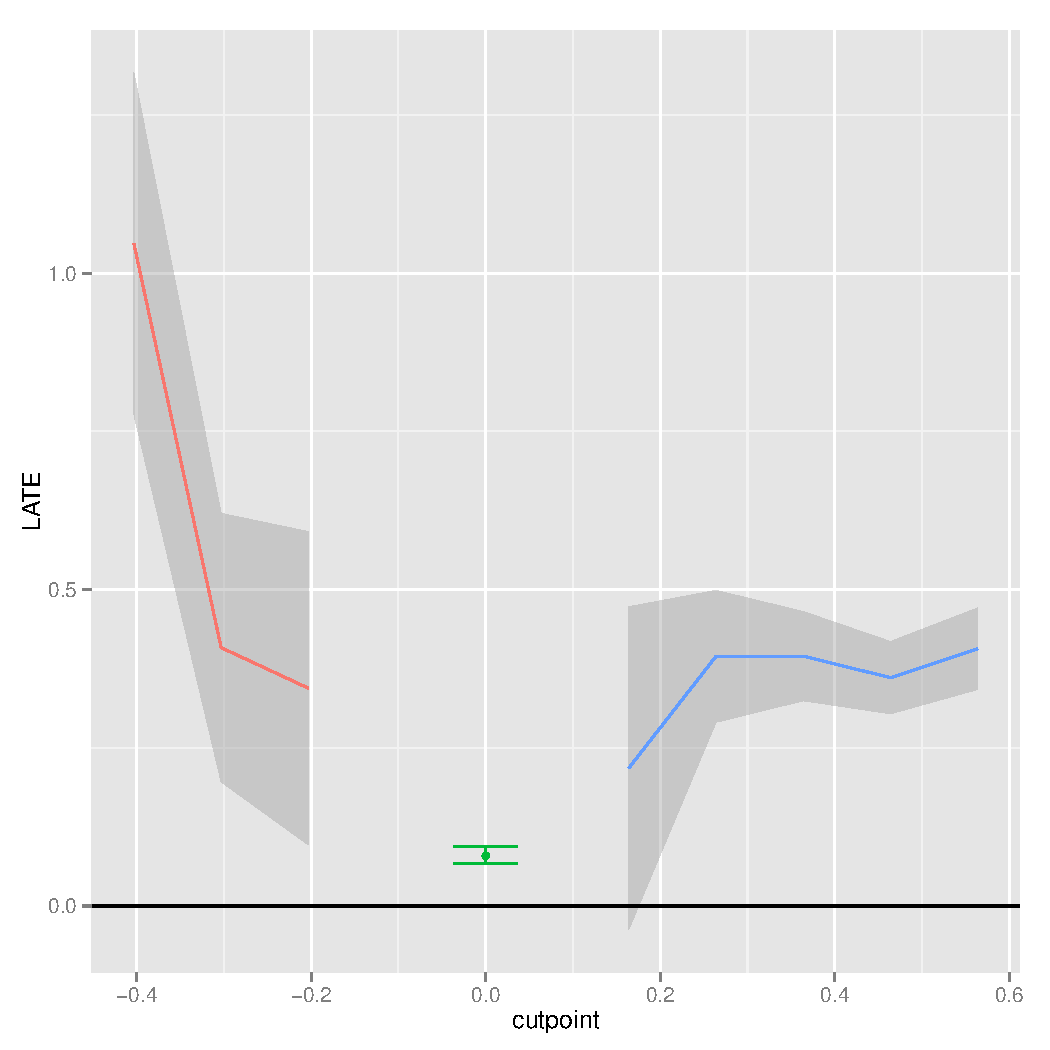
\includegraphics[width=\maxwidth]{figure/unnamed-chunk-15} 

\end{knitrout}



\subsection{Forcing variable}

One of the cases where the assumptions underlying the RDD analysis
might be incorrect is when participants are allowed to manipulate
the variable that lead to treatment, i.e. are able to affect whether
they are treated or not. This question is usually answered factually,
looking at the context of the experiment. One can however also test
whether the forcing variable itself shows a trace of manipulation,
which would result into a discontinuity of its density, as suggested
by \citet{McCrary2008}. 

The test was implemented by D Dimmery in package \pkg{rdd}, and is
simply wrapped by the function dens\_test(), so that it works directly
on a RDDdata object:

\begin{knitrout}
\definecolor{shadecolor}{rgb}{0.969, 0.969, 0.969}\color{fgcolor}\begin{kframe}
\begin{alltt}
\hlkwd{dens_test}\hlstd{(Lee2008_rdd)}
\end{alltt}
\end{kframe}
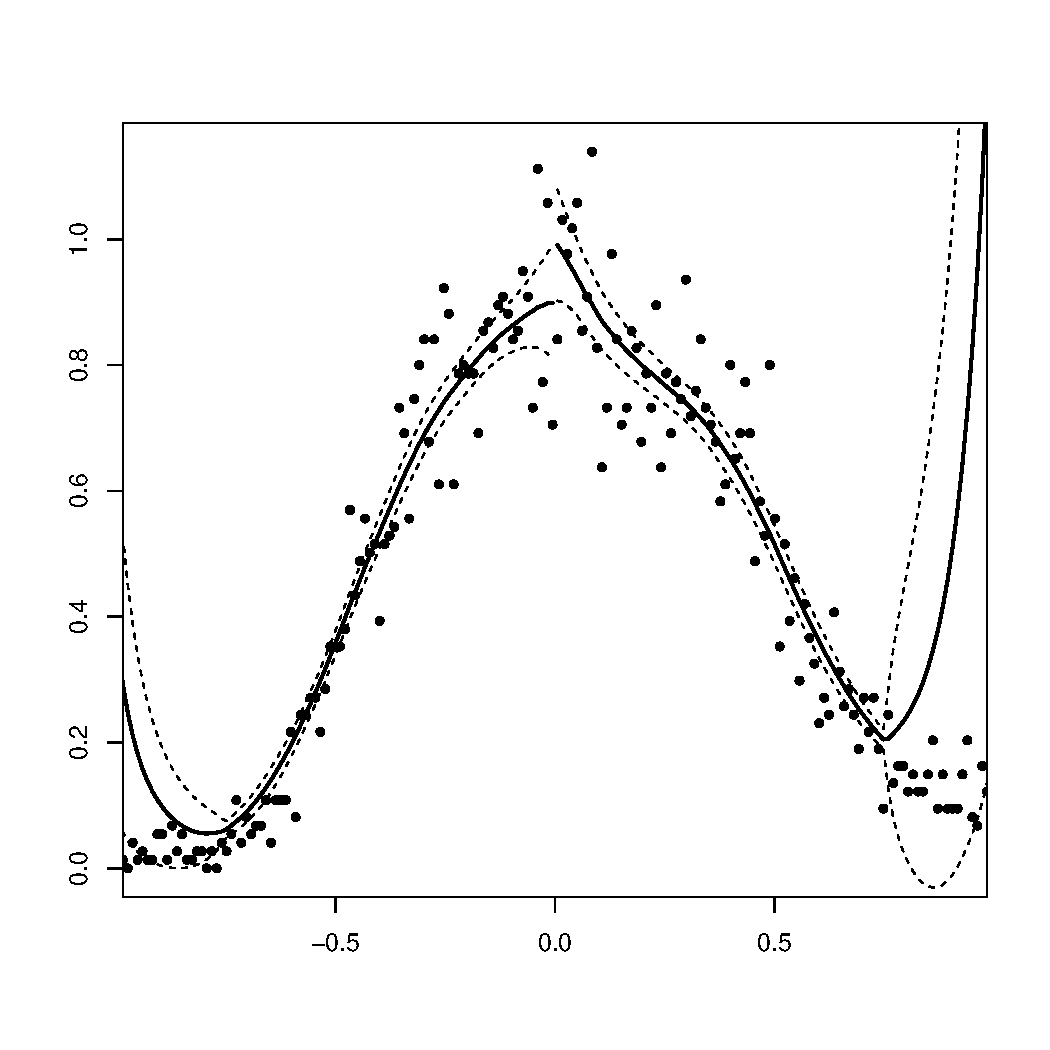
\includegraphics[width=\maxwidth]{figure/unnamed-chunk-16} 
\begin{kframe}\begin{verbatim}
## 
## 	McCrary Test for no discontinuity of density around cutpoint
## 
## data:  Lee2008_rdd
## z-val = 1.295, p-value = 0.1952
## alternative hypothesis: Density is discontinuous around cutpoint
## sample estimates:
## Discontinuity 
##        0.1035
\end{verbatim}
\end{kframe}
\end{knitrout}


The test automatically returns a plot, showing the density estimates
at the left and right of the cutoff, together with the confidence
intervals of these estimates. One rejects the null hypothesis of no
discontinuity if visually the confidence intervals do not overlap. 


\subsection{Baseline Covariates}

Another crucial assumption in RDD is that treatment is randomly distributed
around the cutoff, so that individuals around are similar. This can
be easily tested, as is done in the Randomised Control Trial (RCT)
case, by running test for balanced covariates. Two kinds of tests
have been implemented, allowing to test equality in means (t-test)
or in distribution (Kolmogorov-Smirnov). As this is a typical case
of multiple testing, both functions offers the possibility to adjust
the p-values with various procedures such as the Bonferoni, Holmes
or the more recent Benjamini-Hochberg procedures. 

We run here the equality in means test:

\begin{knitrout}
\definecolor{shadecolor}{rgb}{0.969, 0.969, 0.969}\color{fgcolor}\begin{kframe}
\begin{alltt}
\hlkwd{covarTest_mean}\hlstd{(Lee2008_rdd)}
\end{alltt}
\begin{verbatim}
##    mean of x mean of y Difference statistic p.value
## z1 0.03658   0.01154   -0.02504   1.019     0.3082 
## z2 20.02     20        -0.02255   0.4549    0.6492 
## z3 2.008     2.009     0.001503   -0.07364  0.9413
\end{verbatim}
\end{kframe}
\end{knitrout}


as well as the equality in distribution test:

\begin{knitrout}
\definecolor{shadecolor}{rgb}{0.969, 0.969, 0.969}\color{fgcolor}\begin{kframe}
\begin{alltt}
\hlkwd{covarTest_dis}\hlstd{(Lee2008_rdd)}
\end{alltt}


{\ttfamily\noindent\color{warningcolor}{\#\# Warning: p-value will be approximate in the presence of ties}}\begin{verbatim}
##    statistic p.value
## z1 0.02406   0.3145 
## z2 0.0157    0.8263 
## z3 0.004626  1
\end{verbatim}
\end{kframe}
\end{knitrout}


Since the covariates were generated randomly with a single parameter,
we would expect that no equality test is rejected. 


\section{Conclusion}

\bibliographystyle{econometrica}
\addcontentsline{toc}{section}{\refname}\bibliography{RDD_refs}


%\addcontentsline{toc}{section}{\refname}
%\bibliography{./RDDrefs} 
%\bibliography{/home/mat/Dropbox/Documents/Ordi/Bibtex/GeneralBiblio,/home/mat/Dropbox/Documents/Ordi/Bibtex/biblioFAO_mat} 
\end{document}
